\chapter{Implementación}
\label{chapter:6}

Este capítulo relata el proceso completo de desarrollo del \textit{scraper} para
TvTropes que resuelve los problemas y cumple los objetivos definidos en el
\autoref{chapter:2}. Se siguen uno a uno los distintos hitos que se han ido
alcanzando, explicando por qué son necesarios y las decisiones que se han tomado
en cada uno de ellos para cumplir las historias de usuario, que guían todo el
desarrollo con agilidad.

En este capítulo se irá describiendo el proceso de desarrollo ágil que se ha
llevado a cabo para poder entender cómo se ha llegado a cada uno de los
sucesivos productos mínimamente viables. A lo largo del proceso se justificarán
una serie de decisiones tomadas, buenas prácticas, recomendaciones y
herramientas que permitirán ir refinando el producto hasta llegar a una solución
final de calidad. Esto implica que todos los hitos se desarrollan con el
principal objetivo de satisfacer al usuario y asegurar la calidad, por lo que
conforme se justifiquen las decisiones tomadas para avanzar en cada uno de
ellos, se relacionarán con las historias de usuario definidas, que son las que
confirman qué se debe implementar para cumplir con las expectativas del usuario.

\section{Comienzo del desarrollo}
Con el primer modelado del problema que se ha realizado en el
\autoref{chapter:5}, tenemos definido todo lo necesario para poder comenzar con
el desarrollo y dar una primera versión de un \textit{scraper} que sea capaz de
extraer la información de \textit{tropos} contenida en páginas individuales de
películas de TvTropes. El primer \textit{milestone} de desarrollo es el
\href{https://github.com/jlgallego99/TropesToGo/milestone/3}{M2}, que resuelve
la parte previa a la extracción. Antes de que el \textit{scraper} extraiga la
información que necesita el usuario, que es el objetivo del siguiente hito,
tiene que determinar si la página sobre la que está trabajando es extraíble, es
decir, pertenece a una página de TvTropes que describe una obra con sus
\textit{tropos} y tiene una estructura HTML conocida. Esto permite determinar,
antes de llevar a cabo el proceso de extracción, que el wiki de TvTropes no ha
cambiado demasiado, lo suficiente para saber si el \textit{scraper} programado
sigue funcionando y así evitar procesamiento innecesario. 

Puesto que se está construyendo un producto mínimo, este hito se centra en que
las páginas de obras que se analicen sean solamente de películas, teniendo un
\textit{milestone} futuro dedicado a ampliarlo a otros tipos de medios
audiovisuales. Solo es necesario comprobar y extraer páginas de un tipo de medio
audiovisual concreto para determinar que el \textit{scraper} completa
correctamente sus tareas, ya que el resto de medios consisten en explorar otras
páginas con una estructura similar y que se obtendrán una vez se tenga una araña
que encuentre ese tipo de páginas. Se han elegido páginas de películas por ser
el medio en el que se centran la mayoría de trabajos de investigación estudiados
en la introducción y el estado del arte, y son las que más interés tienen para
una primera versión funcional.

\subsection{Flujo de integración continua para pruebas y compilación}
En este hito se empieza a programar código funcional con lógica de negocio, así
que se comienzan también a desarrollar conjuntamente los tests, concretamente
antes de la propia funcionalidad, tal y como se especifica en el desarrollo
dirigido por pruebas \cite{beck2002driven} y se definió en el
\autoref{chapter:4}. Por tanto, uno de los objetivos de este hito es tener
integrado en el código del proyecto el \textit{framework} de pruebas Ginkgo, que
es el que permitirá desarrollar los tests en Go, para que en los próximos hitos
se puedan desarrollar todas las pruebas para testear las nuevas funcionalidades.
Además, al estar en un entorno de desarrollo ágil la ejecución de las pruebas
estará automatizada, de forma que se tenga un flujo de integración continua que
ejecute automáticamente todos los tests definidos y se pueda comprobar desde el
repositorio de GitHub. 

En cada uno de los hitos, cuando se desarrolla nueva funcionalidad, se abre un
\textit{pull request} en GitHub con los cambios realizados en el proyecto para
saber qué incremento en el producto se está haciendo y qué \textit{issues}
pretende resolver para avanzar en completar el hito. Cada \textit{issue}
representa uno de los sucesivos problemas que surgen durante el desarrollo y que
se intentan resolver para avanzar en completar una historia de usuario. Estos
son los problemas que se justifican y resuelven a lo largo de este capítulo. Los
nuevos flujos de CI que se añaden en este hito permiten automatizar la ejecución
de las pruebas y compilar todo el proyecto, para cumplir que todo el código sea
funcional y asegurar su calidad. Si cualquiera de estos flujos de CI fallan, no
se podrá aceptar el \textit{pull request} y añadir los cambios a la rama
principal. La integración continua en este proyecto se configura mediante
\textit{GitHub Actions}, que automatizan los procesos apoyándose en nuevas
tareas definidas mediante el gestor de tareas \textit{Mask}. Estas tareas
ejecutan los tests para todo el proyecto, ambas usando por debajo la propia
utilidad del lenguaje Go: \texttt{go test} para las pruebas y \texttt{go build}
para comprobar que todos los paquetes del código compilan correctamente. Esto
permite que no haga falta modificarlos en el futuro; servirán para todo el
desarrollo de ahora en adelante y ejecutarán automáticamente todas las nuevas
pruebas que se programen. En el caso de necesitar algún cambio en la ejecución
de los tests o la compilación, bastará con cambiar las tareas del gestor de
tareas, sin necesidad de tocar la configuración de la integración continua.

Por tanto, para poder cumplir con la automatización de las pruebas y la
compilación se configura un nuevo \textit{GitHub Action} en el que se prepara
Go, se instala el gestor de tareas \textit{Mask} y se ejecutan las tareas
definidas para la compilación y el testeo. En un principio se probó a instalar
\textit{Mask} mediante \textit{cargo}, el gestor de paquetes del lenguaje Rust,
ya que la máquina virtual que utiliza el \textit{Action} es de Ubuntu y su
gestor de paquetes no tiene disponible este gestor de tareas en su repositorio
para instalarlo. Sin embargo, esta manera de instalar el gestor de tareas
suponía una gran sobrecarga en el flujo de trabajo al tener que instalar todo el
lenguaje Rust únicamente para instalar un paquete, tardando casi 2 minutos en
ejecutarlo por completo, gastando la mayoría de recursos en instalar el gestor
de tareas. Para solucionar esto se acabó optando por introducir los comandos en
el flujo de CI necesarios para descargar directamente el binario de
\textit{Mask}; esto hizo que se mejorase el tiempo en más de la mitad, ahorrando
los recursos de GitHub y teniendo el resultado del flujo de CI mucho antes.
Adicionalmente, una de las ventajas que tiene el usar Go es que, al ejecutar
cualquier comando de compilación, testeo o ejecución del código, comprueba
automáticamente si las dependencias definidas en el fichero \texttt{go.mod}
están instaladas, y si no lo están las descarga automáticamente, por lo que no
hace falta especificar explícitamente qué dependencias hay que instalar para que
el código funcione.

\subsection{Comprobación de la estructura de una página de TvTropes}
En este hito se modifica el servicio \textit{scraper} añadiendo la funcionalidad
necesaria para cumplir su objetivo: verificar que una página de una obra de
TvTropes no ha cambiado y se puede extraer. Un servicio en DDD hace referencia a
un paquete de código que ejecuta cierta lógica de negocio para un cliente y en
este caso el cliente sería el usuario que necesita los datos. 

El objetivo de este hito se alcanza implementando la función \texttt{CheckValidWorkPage} que 
encapsula la funcionalidad de revisar toda la estructura de una página de
película de TvTropes y validar si el \textit{scraper} podrá extraerla. Recibe
una entidad \textit{Page}, de la cual el \textit{scraper} extrae lo principal
que necesita, que es el URL de la página para poder hacerle una petición y
obtener su código HTML. La razón de recibir la página por referencia se debe a
que la página es mutable, es posible que se haya actualizado y el
\textit{scraper} necesite en el futuro cambiar su atributo de última
modificación, además de que será más eficiente para el \textit{scraper} el
obtener las páginas por referencia que previamente habrá creado el
\textit{crawler} en hitos posteriores. En general, en DDD se tratan las
entidades siempre como referencias, puesto que son mutables, mientras que los
objetos valor se tratarán como variables instanciadas.

Esta función se ha modularizado en distintas subfunciones que realizan
revisiones de distintos tipos, cumpliendo la propiedad de única responsabilidad
de cada una de las funciones y haciéndolas más legibles. Esto facilita que, en
caso de que se necesitasen analizar nuevas partes, se modifiquen las sub
funciones ya existentes o se añada una nueva, que simplemente se llamaría desde
el método principal. Según \textit{clean code} no se deben tener funciones que
mezclen llamadas a otras funciones de alto nivel con lógica más compleja, por lo
que el método principal \texttt{CheckValidWorkPage} se encarga de llamar a las
distintas subfunciones que llevan a cabo verificaciones de distintos tipos y
trata sus resultados para determinar finalmente si la información de la página
es extraíble o no.

Estas comprobaciones se efectúan en orden de menor a mayor complejidad y de
mayor a menor nivel, intentando que el filtrado se lleve a cabo cuanto antes
para evitar entrar en análisis complejos de páginas innecesarias. Se busca poder
validar la página lo antes posible, sin perder mucho tiempo en el proceso para
cumplir la \href{https://github.com/jlgallego99/TropesToGo/issues/45}{[HU06]} lo
mejor posible y que el usuario obtenga cuanto antes el resultado. Primero se
determina si la página pertenece a TvTropes, luego se analiza la estructura
general del artículo principal de la página y finalmente se comprueba la sección
donde deberían estar contenidos los \textit{tropos}.
\begin{itemize}
    \item Para verificar que la página es de TvTropes se extrae el URL de la
    página y se compara si el \textit{host} es \url{tvtropes.org} y si el URI
    corresponde a lo que entendemos como una página de película, es decir,
    pertenece a \textit{Main} y está bajo el índice \textit{Film}. La penúltima
    parte de la ruta tiene que ser el índice al que pertenece la obra, en este
    caso \textit{Film}, y la última parte será el nombre de la película. Esto es
    lo primero que se debe hacer; si la página que se está analizando no es de
    TvTropes y/o no pertenece a una obra, no tiene sentido seguir adelante con
    ella. Sin embargo, puede ser que su estructura interna haya cambiado, por lo
    que es necesario estudiarla más a fondo.
    \item Una vez se sabe que la página es de TvTropes, es necesario ver si
    pertenece a una página de obra y su HTML interno no ha cambiado, ya que es
    de donde luego el \textit{scraper} extraerá la información. Principalmente,
    se revisa en el árbol DOM si la página tiene las partes vistas en el
    análisis de la Figura \ref{fig:tvtropes-work}: un artículo principal con sus
    identificadores y clases conocidas y si el índice, dentro del título del
    artículo, pertenece al de películas. Todas las páginas de obra,
    independientemente de si son películas o no, siguen esta misma estructura,
    por lo que esto basta para confirmar si este tipo de páginas siguen igual.
    \item Por último, se realizan las verificaciones más complejas relacionadas
    con la principal sección que se querrá analizar: la sección de
    \textit{tropos}. Debido al estudio de la Figura \ref{fig:tropelist} del
    \autoref{chapter:5} sabemos que existen tres formas comunes que toma la
    sección de \textit{tropos}, y esto es lo que el \textit{scraper} verifica,
    para asegurarnos de que podemos entender la sección. En este primer hito
    solo se tienen en cuenta los tres tipos, ya que bastan para conformar un
    producto mínimo que sea capaz de analizar la mayoría de páginas de TvTropes,
    sin embargo, en futuros hitos se tendrán en cuenta casos más extremos.\\
    Se sigue la misma estrategia de buscar primero lo más relevante, que en este
    caso es encontrar la sección donde se encuentran los \textit{tropos}, la
    cual está conformada por una lista sin ordenar dentro del artículo principal
    y que está siempre después del resumen y precedida de una etiqueta de
    \textit{header}. Se ignora el comprobar el texto de la cabecera de la
    sección de \textit{tropos}, ya que como se vio en \cite{nishalscraping} el
    contenido cambia mucho y es poco fiable, siendo lo único fiable el hecho de
    que la sección está separada por una cabecera cualquiera. Una vez confirmado
    que la página tiene esa sección, toca ver si se adapta a uno de los tres
    tipos que se conocen. Para probar si los \textit{tropos} están contenidos en
    carpetas basta con buscar el botón de abrir carpetas, que sabemos su
    etiqueta, clase y función JavaScript que utiliza para abrirlas, al estar
    generado siempre igual por el motor del wiki. En todos los casos se valida
    si el primer elemento de la lista es un enlace a una página de
    \textit{tropos} o a una subpágina de ellos. Para este último caso, que
    pertenecería al tercer tipo, se ha hecho uso de una expresión regular que
    confirma si el URI al que redirigen sigue un patrón concreto. Si la última
    parte del URI está codificada como la cadena
    \texttt{/<NombreDeLaObra>/Tropes<XtoY>} entonces se acepta como algo
    conocido. Si la lista contiene cualquier otro elemento inesperado, se
    considera que la página tiene una estructura desconocida y no se puede
    extraer su información.
\end{itemize}

La función de comprobación devuelve un valor booleano, que indica si la página
es extraíble o no, y un error que indica el por qué no es extraíble en caso de
no serlo. En general, es idiomático en Go que todas las funciones devuelvan
siempre un error como último valor para que el código sea autoexplicativo y se
tenga un completo y correcto control de los errores tanto para que las funciones
de testing puedan comprobar todos los casos como para que cualquier cliente que
llame a la función del servicio entienda exactamente qué ha pasado en caso de
error \cite{effective_go}.

Finalmente, en este hito se toma la decisión de que los selectores CSS, los
cuales son una cadena de \textit{string} que hacen referencia a varias etiquetas
HTML y clases, se encapsularán en valores constantes. Esto sigue las guías de
\textit{clean code} sobre evitar los literales, facilitando la legibilidad del
código y evitando la repetición. De este modo, el \textit{scraper} pasará como
parámetro estas constantes a las funciones de Goquery que encuentran los nodos
del árbol DOM de la página que se está explorando. A estas constantes se les da
un nombre lo más semántico posible de forma que el código sea legible y limpio.
Por ejemplo, la constante \texttt{TropeTag} contiene el selector \texttt{a.twikilink} que 
hace referencia a todos los \textit{anchor} de HTML cuya clase es
\textit{twikilink}, que sabemos debido al análisis del capítulo anterior que
hacen referencia a enlaces hacia páginas de \textit{tropos}. El tener constantes
con selectores importantes para lo que quiere buscar el \textit{scraper} también
implica otras ventajas como el poder combinar distintos selectores de modo que
se entienda su significado completo con solo leerlo o el poder adaptarse a los
futuros y posibles cambios que pueda sufrir TvTropes. En el caso de que cambie
alguna clase o etiqueta con la que encontrar alguna sección valiosa de una
página, baste con cambiar la constante y no cambiarlo en cada parte del código
en la que aparezca. En general, al usar constantes semánticas para los
selectores se facilita mucho la legibilidad de algo que de otro modo requeriría
de un análisis más exhaustivo para entender qué significa el selector utilizado,
ya que pueden volverse muy complejos al unir varias reglas.

Se le da en el repositorio de GitHub a esta primera versión del
\textit{software} un etiquetado de versión 0.1.0 que, según las reglas de
versionado semántico\footnote{\url{https://semver.org/}}, hace referencia a que
se añade nueva funcionalidad sin romper lo anteriormente establecido. El primer
número, que indica la versión principal del \textit{software}, se aumentará
cuando se tenga una primera versión completa y funcional de TropesToGo.

\section{Extracción de información en la página principal de una película}
Una vez desarrollada toda la funcionalidad necesaria para comprobar si una
página es de TvTropes y es entendible por el \textit{scraper}, el siguiente paso
lógico es comenzar con el propio proceso de \textit{scraping}, al ser la parte
principal que necesita resolver TropesToGo. La estrategia a seguir en el proceso
de desarrollo es la de centrarse primero en la construcción de uno o más
productos mínimamente viables que culminen en un \textit{scraper} que pueda
sacar toda la información que piden los usuarios según la
\href{https://github.com/jlgallego99/TropesToGo/issues/6}{[HU01]} y
representarlos en un conjunto de datos apto para su uso en procesos de ciencia
de datos, según las historias de usuario
\href{https://github.com/jlgallego99/TropesToGo/issues/30}{[HU05]} y
\href{https://github.com/jlgallego99/TropesToGo/issues/46}{[HU07]}, que
especifican que el usuario necesita acceder al resultado de la extracción en
cualquier momento, de forma offline y en un formato estandarizado. Lo que
produce el \textit{scraper} es el \textit{dataset}; el resultado final que
ofrece TropesToGo al usuario para cumplir sus necesidades, el cual podrá estar
representado en más de un formato ampliamente utilizado por investigadores. Una
vez se tenga un \textit{scraper} totalmente funcional, se podrá avanzar en
futuros \textit{milestones} en el desarrollo de la araña que generalice el
proceso de \textit{scraping} a toda la web de TvTropes completa. 

Por tanto, en este \textit{milestone}
\href{https://github.com/jlgallego99/TropesToGo/milestone/3}{M2} se pretende
ampliar el servicio \textit{scraper} para que pueda extraer los datos presentes
en el artículo principal de varias páginas de prueba. En un principio se tenía
pensado un único hito donde desarrollar el \textit{scraper} completo, capaz de
extraer toda la información necesaria de cualquier película. Sin embargo, al
observar la complejidad que tienen algunas páginas y a lo dispersos que están
los \textit{tropos} de una obra, esa primera idea se dividió en dos productos
mínimos, que son el desarrollado en este hito y en el siguiente. Por tanto, en
este \textit{milestone} el principal objetivo es extraer la información
contenida en la página principal de una película, es decir: su título, año de
salida, índice al que pertenece (el tipo de \textit{media}, o medio audiovisual,
que en este caso será \textit{Film} (película)) y su lista principal de
\textit{tropos}. Existe más información que no se encuentra en el artículo
principal y que se analizará en el siguiente hito, principalmente de
\textit{tropos} adicionales, que está en otras subpáginas de la obra o en
páginas de otros tipos.

Como lista principal entendemos los \textit{tropos} que aparecen directamente
listados al final del artículo, como se podía ver en la figura
\ref{fig:tvtropes-work}, que se consideran los más importantes de la obra al
estar en primer plano. Puesto que este \textit{milestone} está centrado en
extraer información del artículo principal únicamente, se extraerán solo los
\textit{tropos} que están contenidos en listas o carpetas, tal y como se ve en
los dos primeros tipos de la Figura \ref{fig:tropelist}, ignorando por lo pronto
el tercer tipo que, aunque también tiene los \textit{tropos} principales de la
obra, implicaría ahondar en subpáginas. En el próximo \textit{milestone} se
navegará a estas subpáginas y se discutirán las distintas fuentes donde se
pueden encontrar otros \textit{tropos} que no sean los principales.

\subsection{Ampliación del \textit{scraper} para la extracción en el artículo
principal} 

Antes de desarrollar la funcionalidad del \textit{scraper} ha sido necesario
construir la factoría encargada de crear los objetos \textit{Media}, cada uno de
los cuales representa toda la información de una obra de cualquier medio
audiovisual de TvTropes, incluido sus \textit{tropos}. El patrón factoría es uno
de los recomendados en \textit{Domain Driven Design} para la creación de
agregados, y se encarga de formar correctamente el objeto para cumplir la
propiedad de única responsabilidad. Es imprescindible poder generar este tipo de
objetos correctamente, ya que los utilizará el \textit{scraper} para rellenarlos
con los datos extraídos. Por supuesto, de la mano de la creación de la factoría \texttt{Media} 
vienen los tests necesarios, que prueban con varios objetos
válidos e inválidos para comprobar que se cumplen todos los casos definidos y el
manejo de errores es correcto. La factoría, como es común en Go, gestiona una
serie de errores que devuelve como segundo argumento para asegurar siempre que
se conoce el estado de lo que devuelve cualquier método.

En cuanto a la implementación de los métodos que amplían el \textit{scraper}
para darle la funcionalidad de extracción de datos sobre una página web de
TvTropes, se ha seguido una estrategia muy parecida a la seguida en el
\textit{milestone} anterior y según las guías de código limpio
\cite{clean_code_rules}. Se tiene un método principal de \textit{scraping},
encargado de extraer la información relevante de una página de TvTropes
individual, con una separación clara entre la función de alto nivel y las sub
funciones de más bajo nivel a las que llama, encargadas de analizar y extraer
datos de distintas partes de la página.

En general, en el ámbito del \textit{scraping} las tres herramientas más
imprescindibles son: los selectores CSS, que dan operaciones y reglas para
encontrar rápidamente elementos en el HTML de una
página\footnote{\url{https://developer.mozilla.org/es/docs/Web/CSS/CSS_Selectors}};
las expresiones regulares, para identificar patrones y poder tratar mejor las
cadenas de texto fruto de aplicar un selector CSS; y, por último, las
herramientas de desarrollo del navegador web, para analizar el HTML interno de
una página, encontrar las partes fundamentales que se quieren extraer y probar los
selectores CSS en ella para comprobar que apuntan justo a los recursos deseados.

Para extraer el título, el índice y el tipo de medio audiovisual de la página de
una obra (en este caso, solo obras que son películas) se han empleado los mismos
selectores que en la comprobación de la página y que se vieron en el análisis de
la estructura de TvTropes, que apuntan directamente al \textit{header} del
artículo que tiene toda esta información. En este caso, puesto que queremos la
información y no basta con verificar, se ha hecho uso de una expresión regular
que separa las tres partes que queremos, que es capaz de identificar cualquier
año en mitad de una cadena de texto. Sin embargo, el principal problema a la
hora de extraer información en el artículo principal ha estado relacionado con
los \textit{tropos}. En un principio se tenía ideado el extraer solamente los
\textit{tropos} que figuran en la lista, como cabeza de cada uno de los
elementos de ella, y también aquellos a los que se hace referencia en las
descripciones de ellos y en el resumen de la película. El problema de esto es
que se han encontrado casos de \textit{tropos} que, cuando están referenciados
en mitad de un texto y no como un elemento principal de la lista, no pertenecen
necesariamente a la obra. En algunos casos se referencian como ejemplo de
\textit{tropo} contrario o cualquier otra razón, lo que hace que no se pueda
determinar si pertenecen como tal a la obra o no, así que se descartan. Por
tanto, se hace un cambio de estrategia en el que se considera que, para este
\textit{milestone}, los \textit{tropos} que se extraen son únicamente los que
aparecen en cada elemento de la lista o carpetas, que se consideran
``principales''.

Ha sido necesario construir dos selectores CSS nuevos, apoyándose en las guías
de Mozilla para selectores, que permitan seleccionar fácilmente y de manera
exclusiva los \textit{tropos} principales, tras un proceso de análisis de la
página mediante el inspector de elementos HTML del navegador. Cada uno de estos
selectores condensan en una sola instrucción todo lo necesario para encontrar
cada uno de los enlaces a \textit{tropos} que encabezan cada elemento de la
lista, tanto para una lista simple como para el caso de que estén en carpetas.
Como se vio en la figura \ref{fig:tvtropes-work}, cuando TvTropes define los
\textit{tropos} de una obra, siempre los muestra en una lista donde cada primer
elemento es un hipervínculo con estructura conocida y fácilmente identificable.
Por supuesto, al igual que en el hito anterior, se construyen los selectores
como \textit{strings} constantes con un nombre legible, de forma que se eviten
utilizar literales en el código y sea más legible.

Por tanto, se obtienen inequívocamente los \textit{tropos} de una lista simple
en el artículo principal de una obra de TvTropes mediante el selector CSS de la
Figura \ref{fig:selector-lista}.

\begin{figure}[ht]
    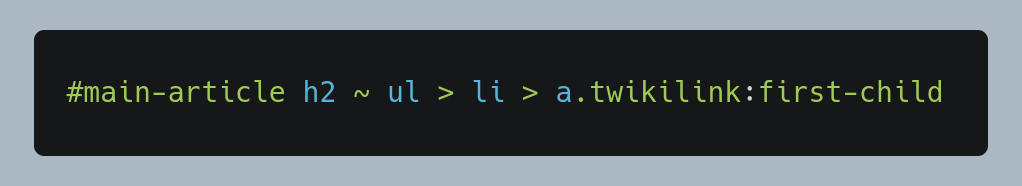
\includegraphics[width=\textwidth]{img/selector-tropes.png}
    \caption{Selector CSS para extraer todos los \textit{tropos} principales de
    la lista simple.}
    \label{fig:selector-lista}
\end{figure}

La primera parte es común en otras funciones del \textit{scraper}, ya que busca
el artículo principal, que es donde siempre va a estar toda la información que
necesitamos, y luego busca el \textit{header} que siempre precede a la sección de
\textit{tropos} independientemente de la página. Una vez hecho esto, se hace uso
del combinador general de hermanos
\begin{otherlanguage}{english}(representado por el símbolo
\textasciitilde)\end{otherlanguage} para seleccionar los elementos HTML que
están al mismo nivel; en este caso, identifica todos los primeros elementos de
lista \texttt{<ul>} que son hermanos de la cabecera que da inicio a la sección
de \textit{tropos}. Se recuerda que, aunque visualmente en la página parezca una
sola lista, internamente suele estar partida en distintos elementos \texttt{<ul>} 
al mismo nivel, por lo que esto nos permitiría seleccionar todos
ellos. Con esto ya tenemos identificada sin lugar a equivocaciones la sección de
\textit{tropos}. A continuación, se emplea dos veces el combinador de hijo
\begin{otherlanguage}{english}(representado por el símbolo
\textgreater)\end{otherlanguage}, que escoge aquellos elementos que sean hijos
directos del primer elemento. Partiendo de que se tiene seleccionada la lista
principal, en la primera combinación se buscan todos sus hijos directos, que son
cada uno de los elementos \texttt{<li>} de la lista, y en la segunda se busca el
siguiente hijo directo, que es la primera etiqueta que encabeza cada punto de la
lista. Esta etiqueta es ya el hipervínculo al \textit{tropo} que queremos. Al
final, se indica la pseudo clase \texttt{:first-child} para indicar que
únicamente queremos el primer enlace de \textit{tropos} \texttt{a.twikilink} que
aparezca. De esta manera se ignoran aquellos enlaces que no queremos, que son
los que aparecen referenciados en la descripción de cada \textit{tropo}
principal, y solo nos quedamos con el que encabeza cada punto de la lista.

Este selector completo también resuelve uno de los principales problemas que se
han encontrado al intentar extraer los \textit{tropos}. Existen muchos casos en
los que un elemento de la lista de \textit{tropos} contiene sublistas con
descripciones adicionales y \textit{tropos} que no queremos, al ser
referenciados en la descripción y no principales. En primeras versiones del
selector se llegaba a meter en esas sublistas, sin embargo, se pudo resolver
gracias al combinador general de hermanos, que únicamente selecciona las listas
que estén al mismo nivel, evitando meterse en sublistas. 

En cuanto al selector para los \textit{tropos} que se encuentran en carpetas, en
la \ref{fig:selector-folder}, es muy parecido al anterior pero con una ligera
diferencia necesaria. Aunque dentro de las carpetas lo que se tenga es una
estructura HTML idéntica al caso en el que no haya carpetas, distintos elementos \texttt{<ul>} separados 
arbitrariamente donde cada elemento es un \textit{tropo}, el que es hermano de
la cabecera de la sección de \textit{tropos} en este caso no es un elemento \texttt{<ul>} sino 
la carpeta. Por eso, en este caso, el selector se simplifica,
buscando únicamente los hijos directos de la carpeta, sin necesidad del selector
de hermanos. Esto también evita las sublistas, porque no son hijos directos de
la carpeta.

\begin{figure}[ht]
    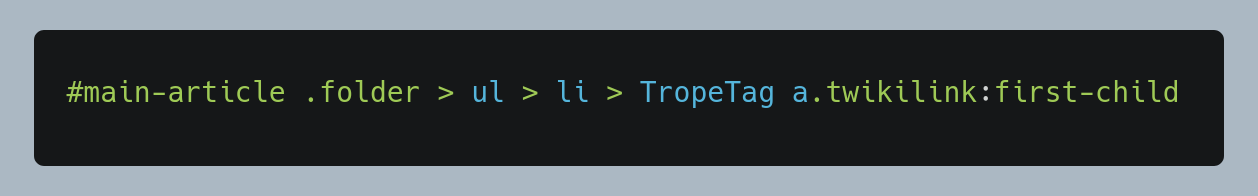
\includegraphics[width=\textwidth]{img/selector-tropes-folders.png}
    \caption{Selector CSS para extraer todos los \textit{tropos} principales en
    carpetas de listas.}
    \label{fig:selector-folder}
\end{figure}

El resultado final de ambos selectores es, por tanto, todas las etiquetas de
hipervínculo que indican un \textit{tropo} principal. Estas tienen los dos datos
necesarios para el \textit{scraper}: el nombre del \textit{tropo}, dentro de la
propia etiqueta, y su URI en el elemento \texttt{href} para poder dirigirse a
esa página si fuese necesario.

Con esto ya estaría desarrollada la parte del \textit{scraper} correspondiente a
este hito, que se encarga de extraer toda la información de una página y
construir el objeto con la información de la página con sus \textit{tropos}.
Cabe destacar que para implementar la estructura de datos que maneja los
\textit{tropos} de una obra se ha utilizado un set, ya que es una estructura de
datos en la que todos sus elementos son únicos, y en una obra no tiene sentido
que existan \textit{tropos} repetidos. Finalmente, se desarrollan sin problema
los tests que comprueban que el resultado de la extracción es correcto,
comprobando si el título, año y URL son los esperados y si en el set todos los
objetos hacen referencia a \textit{tropos} reales y no están repetidos. Estos
tests se realizan con varias páginas de TvTropes de prueba que tienen los
\textit{tropos} en listas y en carpetas. Una vez hecho esto, el próximo paso
para completar este hito es poder trasladar esta información a un
\textit{dataset}.

\subsection{Implementación de repositorios para manejar los \textit{datasets}}
Finalmente, la última parte que resta para completar este hito es el
almacenamiento de uno o varios objetos \texttt{Media} en un conjunto de datos
con un formato estandarizado. Recordamos que estos objetos son agregados que
representan una obra con sus \textit{tropos}. Los repositorios son los
encargados en DDD de persistir los agregados y, como se vio en el modelado
inicial del problema, se modela un repositorio para este tipo de objetos.

En la interfaz repositorio de \texttt{Media} se describen únicamente aquellos métodos
genéricos que cumplan las necesidades del usuario. La principal funcionalidad es
la de poder añadir objetos \texttt{Media} al \textit{dataset}, ya que según la
\href{https://github.com/jlgallego99/TropesToGo/issues/6}{[HU01]} y la
\href{https://github.com/jlgallego99/TropesToGo/issues/30}{[HU05]}, el usuario
quiere la totalidad de los datos extraídos en un único \textit{dataset}, y que
según la \href{https://github.com/jlgallego99/TropesToGo/issues/46}{[HU07]}
quiere poder tenerlo en cualquier momento, por lo que tiene que ser un conjunto
de datos persistido en memoria, en un fichero al que pueda acceder. Además de
esto, también se debe poder actualizar el conjunto de datos debido a la
naturaleza cambiante de los datos en TvTropes, y el usuario pide tener la
versión más reciente de la información, tal y como indica la
\href{https://github.com/jlgallego99/TropesToGo/issues/9}{[HU04]}. Por otro
lado, métodos que suelen ser típicos de implementaciones CRUD, como la lectura
del repositorio, no tienen sentido que las ofrezca el \textit{scraper}. El
usuario no va a utilizar este \textit{software} para leer los datos, sino para
que le genere un conjunto con ellos que ya utilizará en la manera que crea
necesario y, por tanto, solo son necesarias funcionalidades de creación, borrado
y actualización.

Esta definición genérica de la interfaz repositorio permite poder implementar en
cualquier momento \textit{structs} que, implementando todos los métodos de la
interfaz, definan una nueva forma de persistencia de los datos extraídos. Esto
garantiza la propiedad de extensibilidad del código y está en consonancia con la
\href{https://github.com/jlgallego99/TropesToGo/issues/30}{[HU05]}, donde se
especifica que el usuario quiere poder elegir el formato en el que se represente
el conjunto de datos de entre los más comunes en ciencia de datos. El
representar los repositorios del conjunto de datos como algo genérico, con una
misma definición, permite tener en cuenta en todo momento esta historia de
usuario para añadir nuevos formatos soportados por TropesToGo en caso de
necesitarlos y luego poder reutilizarlos fácilmente. Para seguir esta HU y
cumplir este hito, se implementan dos repositorios de \texttt{Media} para
\textit{datasets} en formato CSV y JSON. El formato CSV es el más frecuente en
cualquier tarea de ciencia de datos y tiene la ventaja de que es independiente
del lenguaje. Por su parte, el JSON tiene las mismas ventajas, estando presente
en multitud de ámbitos como formato para representación de datos, como por
ejemplo en API REST, y es el formato de los datos de Tropescraper.

En cuanto a la información que tiene que contener el \textit{dataset}, ya la
conocemos, puesto que son todos los campos que contiene cada objeto \texttt{Media} 
en los que, sin embargo, la forma de representación varía entre
los formatos de datos. En general, en el fichero de datos tienen que figurar una
serie de entradas, una detrás de otra, que representen una obra y toda su
información relevante. Esta información es: tanto el título como el año de la
obra, para identificarla inequívocamente
(\href{https://github.com/jlgallego99/TropesToGo/issues/8}{[HU03]}), su URL de
TvTropes, la fecha en la que se actualizaron sus datos por última vez, el tipo
de medio audiovisual al que pertenece (para este hito, de momento solo
películas) y su lista de \textit{tropos}, donde cada \textit{tropo} es una tupla
de su nombre y su índice. 

El índice al que pertenece un \textit{tropo} hace referencia al tipo o
papel que tiene en la narrativa de una historia; pueden ser narrativos, de
género, sobre temas específicos, etc. y es una decisión guiada por la
\href{https://github.com/jlgallego99/TropesToGo/issues/57}{[HU08]}. El usuario
necesita esta información para poder realizar análisis más complejos en los que
se entiendan las relaciones entre \textit{tropos} al conocer de forma objetiva
para qué se utilizan. La extracción de esta información no se hace en este
hito, se delega a un \textit{milestone} posterior, ya que es información de
metadatos secundaria que no es imprescindible para construir este producto
mínimo, sin embargo, el hecho de que exista se tiene en cuenta desde el
principio.

Los repositorios para JSON y CSV se implementan en paquetes separados, para
preservar el principio de única responsabilidad, y definen únicamente las
funciones necesarias. Por tanto, se tienen módulos de repositorio completamente
desacoplados, que únicamente reciben un objeto \texttt{Media} con el cual
efectuar sus operaciones. Se puede ver un ejemplo de cómo estaría representada
la información completa de una obra en la Figura \ref{fig:json-dataset} para el
\textit{dataset} JSON y en la Figura \ref{fig:csv-dataset} para el conjunto de
datos CSV. En el caso de JSON se tiene una clave principal ``tropestogo'', que
contiene un array con todos los resultados del \textit{scraping}. Cada uno de
los objetos contiene toda la información principal en el mismo nivel, y los
\textit{tropos} son un array cuya información anidada contiene su título y su
índice. En el fichero CSV cada dato es una columna, sin embargo, para
representar los tropos y sus índices se ha tenido que separar en dos columnas
distintas. Dentro de esas columnas se tiene de igual manera un array, donde cada
elemento está separado por punto y coma (un delimitador distinto que el que
separa entre columnas, que es la coma), y la posición en un array se corresponde
con la del otro, para relacionar el nombre del \textit{tropo} con su índice.

\begin{figure}[ht]
    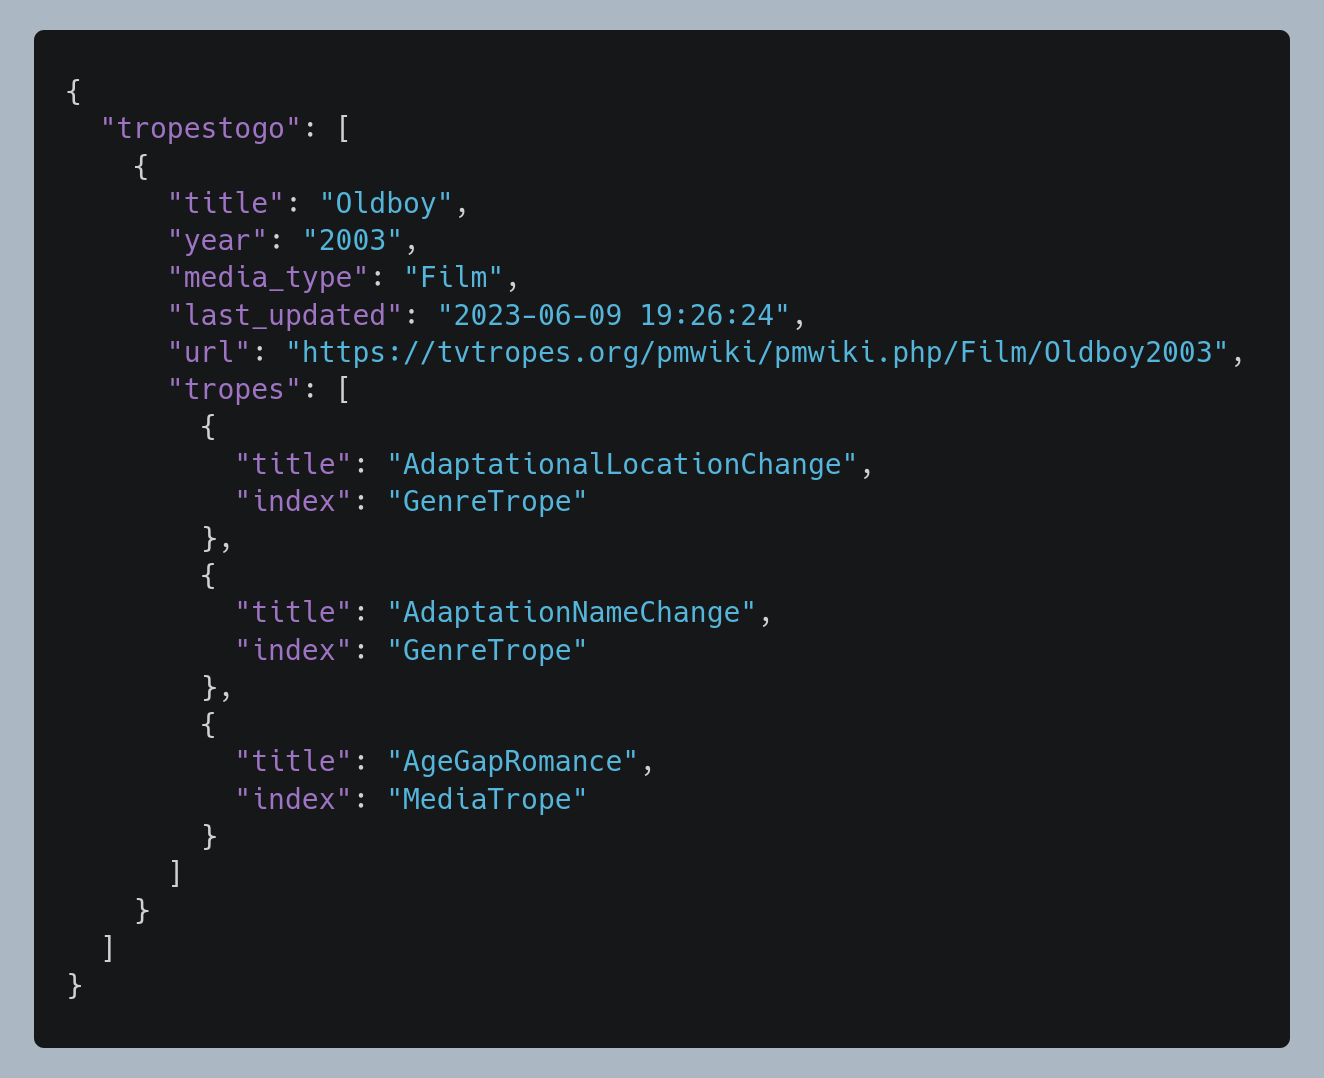
\includegraphics[width=\textwidth]{img/dataset-json.png}
    \caption{Ejemplo de representación de los datos de una película de TvTropes en JSON.}
    \label{fig:json-dataset}
\end{figure}

\begin{figure}[ht]
    \begin{table}[H]
        \begin{tabular}{|l|l|l|}
        \hline
        title         & year & lastupdated         \\ \hline
        Oldboy (2003) & 2003 & 2023-06-09 19:26:24 \\ \hline
        \end{tabular}
    \end{table}
    \begin{table}[H]
        \begin{tabular}{|l|l|}
        \hline
        url                                                    & mediatype \\ \hline
        https://tvtropes.org/pmwiki/pmwiki.php/Film/Oldboy2003 & Film      \\ \hline
        \end{tabular}
    \end{table}
    \begin{table}[H]
        \begin{tabular}{|l|}
        \hline
        tropes                                                        \\ \hline
        AgeGapRomance;AdaptationalLocationChange;AdaptationNameChange \\ \hline
        \end{tabular}
    \end{table}
    \begin{table}[H]
        \begin{tabular}{|l|}
        \hline
        tropes\_index                    \\ \hline
        MediaTrope;GenreTrope;GenreTrope \\ \hline
        \end{tabular}
    \end{table}
    \caption{Ejemplo de los campos que tiene un \textit{dataset} de TvTropes en CSV.}
    \label{fig:csv-dataset}
\end{figure}

Para tratar con los ficheros en JSON ha sido necesario implementar la interfaz
\textit{Marshaler} de la biblioteca estándar de Go, ya que es obligatorio si se
quieren codificar y descodificar objetos complejos a JSON. Con esto ya se tiene
una forma sencilla de transformar objetos entre el fichero JSON y las
estructuras internas del código. En el caso de CSV es más sencillo debido a que
la biblioteca estándar de CSV de Go contiene una función para escribir sobre
este tipo de ficheros. En general, el CSV es más fácil de tratar, puesto que es
un formato muy sencillo que consta únicamente de líneas una detrás de otra, más
fáciles de tratar con los métodos convencionales de escritura y lectura de
ficheros. 

Se sigue una misma estrategia en ambos repositorios para facilitar la gestión de
los datos y para reducir lo máximo posible el número de lecturas y escritas en
ficheros, que pueden comprometer bastante la eficiencia (en relación con la
\href{https://github.com/jlgallego99/TropesToGo/issues/45}{[HU06]}). El flujo
general de funcionamiento de los repositorios consiste en que, al añadir un
nuevo objeto \texttt{Media} correctamente formado, no se persiste directamente,
sino que se almacena en un vector de objetos \texttt{Media} como parte del
objeto \textit{scraper}. Este vector se va rellenando con las sucesivas llamadas
de añadir objetos \texttt{Media} hasta que finalmente se decida llamar a un
método que se encarga de volcar (persistir) todos los datos de la variable en
memoria al fichero, vaciando la memoria y construyendo todo el \textit{dataset}
en una sola vez.

Los métodos de borrado y actualización siguen una filosofía muy parecida en
ambas implementaciones. El borrado se ha implementado como una limpieza completa
del dataset, para ayudar en la regeneración de conjuntos de datos al testear,
eliminando todo registro, tanto en memoria como en el \textit{dataset}, y
dejando únicamente la cabecera de las columnas en el CSV o la clave principal
con un array vacío en el JSON. La actualización por su parte consiste en un
proceso de carga de todo el \textit{dataset} del fichero en una variable
temporal, lo cual permite tratar más fácilmente los datos en términos propios
del lenguaje. Para esto, en el caso de JSON basta con realizar una
decodificación del JSON a las estructuras de datos de Go que contienen los
datos, haciendo la actualización como una búsqueda simple en el array de objetos \texttt{Media} 
y modificando lo necesario. Al llevar a cabo las modificaciones sobre los
objetos internos, se vuelve a escribir todo el conjunto de datos, terminando la
actualización. Este es un proceso que está pensado solamente en el caso de que
el \textit{scraper} encuentre datos más actualizados, para no tener que volver a
generar todo el conjunto, sino únicamente actualizar el objeto que se quiere.

Por su parte, el añadir datos nuevos consiste únicamente en añadir de forma
intermedia el objeto \texttt{Media} al vector en memoria, comprobando
previamente que no es repetido, quedándose ahí hasta que se decida persistirlo.

Adicionalmente, en este hito se ha tomado la decisión de replantear un poco el
modelado DDD de las páginas de TvTropes. Modelar una única página como una
entidad es insuficiente para hacer relaciones correctas y tiene más sentido como
un objeto valor que, además de su URL, que es lo principal, describa también qué
tipo de página de TvTropes es. Saber si la página es de una obra, \textit{tropo}
o índice permitirá al \textit{scraper} y al \textit{crawler} en el futuro
trabajar de una manera más rápida y sencilla. Ahora, para representar todas las
páginas de TvTropes, se utiliza una entidad \texttt{TvTropesPages} que se
encarga de gestionar la creación y mantenimiento del conjunto de todas las
páginas encontradas en TvTropes, donde el objeto valor \texttt{Page} es el
identificador de cada página, que están relacionados directamente por hash (en
una estructura \textit{map}) con su fecha de última actualización. Esta entidad
controla la creación de las páginas y da la posibilidad de modificar su fecha de
actualización. 

Por último, a lo largo del desarrollo de este \textit{milestone} se detecta un
problema importante que es necesario resolver para terminar este PMV: los tests
del \textit{scraper} del hito anterior funcionaban haciendo peticiones HTTP
directamente a TvTropes. Esto interfiere directamente con cómo deberían ser las
pruebas unitarias, que deberían únicamente confiar y usar los recursos
propios del proyecto. Que los tests dependan de si TvTropes está funcionando, de
la velocidad de la red, o incluso de arriesgarse a ser vetado de la página o con
peticiones limitadas por tiempo, puede dificultar los tests de la lógica interna
del \textit{scraper}, que deben poder ejecutarse y funcionar independientemente
de si TvTropes está disponible en ese momento o no.

Para resolver esto, se realizan pequeños cambios en el planteamiento del
\textit{scraper}, dejando el análisis de la página como una subfunción de la
que recibe una entidad página y realiza una petición HTTP a TvTropes. A partir
de ahora se emplearán, únicamente para los tests, ficheros HTML descargados
directamente de TvTropes y guardados en el repositorio. Esto supone una
consideración adicional que ya se discutió en el \autoref{chapter:3}; los
contenidos de TvTropes están bajo una licencia
\begin{otherlanguage}{english}\textit{Creative Commons
Attribution-NonCommercial-ShareAlike 3.0
Unported}\end{otherlanguage}\footnote{\url{https://CreativeCommons.org/licenses/by-nc-sa/3.0/}},
la cual permite redistribuir sus contenidos siempre que sea de forma no
comercial, con la misma licencia y dando crédito al autor original. Puesto que
descargar y trabajar directamente con el HTML de algunas páginas TvTropes entra
dentro del uso de esta licencia, se añade al repositorio de GitHub, se informa
de su uso y se da crédito a TvTropes como los autores de ese contenido.
 
Ahora el análisis de una página de TvTropes trabaja directamente sobre cualquier
objeto genérico que contenga el HTML de la página, siendo el cómo se obtiene ese
objeto un paso previo que se queda encapsulado en una función previa que realiza
peticiones HTTP y llama a esta función de análisis. Por tanto, los tests pueden
directamente llamar a esta función de análisis cargando desde el test el fichero
HTML que se tiene en disco. Esta nueva manera de enfocar los tests nos permite
evitar los problemas de red poder testear más en profundidad los contenidos de
una página, ya que al estar persistida en disco sabemos que no va a cambiar, y
confirmar así que la lógica del \textit{scraper} es correcta.

Se le da en el repositorio de GitHub a esta nueva versión del \textit{software}
un etiquetado de versión 0.2.0 que, según las reglas de versionado
semántico\footnote{\url{https://semver.org/}}, hace referencia a que se añade
nueva funcionalidad sin romper lo anteriormente establecido. En general, lo que
se hace es aumentar y mejorar la funcionalidad del \textit{scraper}.

\section{Extracción de información en las subpáginas de una película}
En TvTropes las páginas se organizan en espacios de nombres, y uno de esos
espacios de nombres son las sub
wikis\footnote{\url{https://tvtropes.org/pmwiki/pmwiki.php/Main/SubWiki}}, o sub
páginas de una obra, que presentan información más centrada en un tema concreto.
Cada obra tiene una serie de subpáginas temáticas muy variadas; no todas tienen
las mismas, pero siempre se hacen referencia en ellas a \textit{tropos} que, en
muchos casos, no están en la parte principal. En muchos casos estos
\textit{tropos} se consideran demasiado subjetivos y dependen del criterio del
miembro de la comunidad que los ha identificado, como por ejemplo los del
espacio de nombres YMMV. Por estas razones, podemos hacer una distinción entre
los \textit{tropos} de una obra que son principales, al estar listados en el
artículo principal, y secundarios, al pertenecer a una o más subpáginas
temáticas dentro de una obra. A continuación, se resuelve el segundo producto
mínimamente viable relacionado con la extracción de \textit{tropos} de una obra,
que tendrá ya el desarrollo mínimo de un \textit{scraper} para TvTropes con el
que poder pasar a trabajar en la araña. Por tanto, en este hito se abordará el
proceso de desarrollo y ampliación del \textit{software} para la extracción de
\textit{tropos} en subpáginas. Esto aumentará el número de \textit{tropos} que
TropesToGo es capaz de identificar, organizando cada vez más la información tan
distribuida que tiene TvTropes. Todo este desarrollo sigue motivado
principalmente por la
\href{https://github.com/jlgallego99/TropesToGo/issues/6}{[HU01]}, que nos pide
obtener todos los \textit{tropos} de todas las obras de la web, y se tendrá una
solución que mejore la extracción que realizaba Tropescraper, que se centraba
únicamente en los \textit{tropos} principales.

\subsection{Ampliación del \textit{scraper} para extraer todos los \textit{tropos} principales en subpáginas}
Antes de pasar a la extracción en los subwikis, es necesario ampliar el
\textit{scraper} con lo último necesario para que sea capaz de obtener los
\textit{tropos} principales de todo tipo de páginas. En el hito anterior se
obtuvieron aquellos ordenados en cualquier tipo de lista o carpetas, y quedaba
por ver el último tipo de la Figura \ref{fig:tropelist} en el que, cuando los
\textit{tropos} principales son demasiados, se dejan fuera del artículo
principal y es necesario explorar subpáginas que los dividen y ordenan
alfabéticamente.

Estas subpáginas con \textit{tropos} principales siempre siguen las mismas
reglas, que han facilitado su extracción:
\begin{itemize}
    \item Los enlaces a ellas se encuentran siempre donde está la sección de
    \textit{tropos}. En este caso, la lista contiene únicamente enlaces a sub
    páginas de diversos tipos, pero no necesariamente principales, sino también
    temáticas con \textit{tropos} secundarios. En la Figura \ref{fig:tropelist3}
    se puede ver un ejemplo de esto, donde se dan enlaces a dos subwikis
    distintas de lo principal. 
    \item Se identifica cuándo un enlace es a una subpágina de \textit{tropos}
    principales con una simple expresión regular que compruebe que las dos
    últimas partes del URI son: primero, el título de la obra, y segundo, una
    cadena del tipo
    \begin{otherlanguage}{english}``TropesXtoY''\end{otherlanguage}, donde X e Y
    son cualquier letra mayúscula, que indican el rango alfabético de
    \textit{tropos} que presentan.
    \item La estructura de cada una de estas subpáginas es idéntica a la de una
    página típica de obra, solo que únicamente conteniendo la parte de
    \textit{tropos}.
    \item Los \textit{tropos} se presentan en cualquiera de las dos formas
    vistas anteriormente: listas o carpetas, con el \textit{tropo} principal
    encabezando cada elemento de la lista.
\end{itemize}

Por tanto, para realizar esta extracción se ha utilizado una estrategia simple
reutilizando el método que extrae los tropos del anterior milestone. Este método
era capaz de, como sabemos, extraer todos los tropos presentes en cualquier
artículo principal siempre que estuviesen en listas o carpetas. Puesto que esta
misma estructura de a veces carpetas a veces listas. Por tanto, para solucionar
esto basta con lanzar esta función general de tropos tantas veces como sub
páginas se encuentren, formando listas parciales de \textit{tropos} por cada sub
página y formando una lista final sumando todas ellas. Ahora, cuando el
\textit{scraper} extrae información de una página de obra y llega a la sección
de \textit{tropos}, comprueba si estos están en subpáginas o no, y según eso
sigue una de las dos estrategias.

\subsection{Responsabilidad única del \textit{scraper} y uso de \textit{readers}
para testing} 

Adicionalmente, se llevan a cabo varios retoques del servicio \textit{scraper}
para hacerlo más funcional, que sus métodos estén más centrados en una única
funcionalidad y en general tener el código más limpio, claro y documentado.

Para poder tener un producto mínimo viable más adecuado, y garantizar la propiedad de
única responsabilidad del \textit{scraper}, se vuelve a dar un pequeño
cambio, pero importante, a la entidad \texttt{TvTropesPages} que modela todas las
páginas que se encuentren en TvTropes. El \textit{scraper} debe encargarse
únicamente de extraer información de páginas que se le ofrezcan, es decir, la
responsabilidad de buscar las páginas y sus subpáginas no recae en él, sino en
el \textit{crawler}. Todas las funciones del \textit{scraper} deben, por tanto,
trabajar con esta entidad o con objetos valor página de forma individual,
únicamente sacando datos, formando objetos \texttt{Media} correctos y manejando
sus repositorios (los \textit{datasets}) para que los clientes hagan lo
pertinente con ellos.

Se crea una entidad \texttt{TvTropesSubpages} que relaciona mediante un
\textit{map} una serie de subpáginas con sus respectivas fechas de última
actualización para satisfacer la
\href{https://github.com/jlgallego99/TropesToGo/issues/9}{[HU04]}. De igual
manera, para poder modelar cada página con sus subpáginas, se relacionan
mediante un \textit{map} en la entidad \texttt{TvTropesPages} cada página
(objeto valor \texttt{Page} que representa una página de cualquier tipo), con la
entidad de las subpáginas. De esta manera, se modela una entidad que
gestiona y relaciona todas las páginas, sus subpáginas y las fechas de última
actualización de todas ellas. Esta es la principal entidad con la que se quiere
que trabaje el \textit{crawler}, al encontrar las páginas que luego se quiere
que extraiga el \textit{scraper}.

Adicionalmente, se modifican todos los métodos de extracción para que trabajen
con objetos \textit{reader} de la biblioteca de entrada/salida de Go. Un
\textit{reader}\footnote{\url{https://pkg.go.dev/io}} representa cualquier flujo
de datos de lectura, y es el tipo de datos que acepta Goquery para formar el
árbol DOM con el que trabaja el \textit{scraper}. La ventaja de definir los
parámetros de las funciones del \textit{scraper} como \textit{readers} es que el
contenido HTML puede venir de cualquier fuente, ya sea de haberlo obtenido tras
una petición HTTP o de leer un fichero local en disco. Por tanto, ahora se tiene
un método general que se encarga de realizar todas las llamadas a los distintos
métodos que hacen el \textit{scraping} de las distintas partes de una página,
para todas las páginas, pero donde el reader es el HTML obtenido de hacer una
petición HTTP a TvTropes. Para los tests, se llama directamente a cada uno de
los métodos para testearlos, dándoles como parámetro un \textit{reader} con el
contenido de la página HTML que se tiene guardada en disco, para seguir
garantizando que los tests funcionen en cualquier ámbito y sin depender de
factores externos.

Esto conforma una nueva versión del \textit{software} funcional, con 0.3.0 como
número de versión, indicando que ha habido una mejora con nueva funcionalidad.
Concretamente, esta nueva funcionalidad es la posibilidad de extraer
\textit{tropos} principales en subpáginas.

\subsection{Extracción general de \textit{tropos} en los subwikis para todos los espacios de nombres}
Previo a esta extracción, se modifica el objeto valor \texttt{Trope} para
reflejar dos nuevos campos: si es principal y, si no lo es, a qué subwiki (o
espacio de nombres) pertenece. Esto pone de manifiesto aún más la ventaja de
tener los \textit{tropos} modelados como objetos valor, ya que pueden
representar más sencillamente estos campos. Puesto que los objetos valor son
inmutables y se instancian, un mismo \textit{tropo} puede estar instanciado dos
veces en dos obras distintas, porque en una puede ser principal y en otra no,
por ejemplo. En general, los \textit{tropos} se modelan como algo que siempre
nos dice lo mismo, pero siempre dentro del contexto de cada obra. Este modelado
nos permitirá organizar y representar mejor los \textit{tropos} que se extraen
con esta ampliación del \textit{scraper}.

El \textit{scraper} no debe realizar ninguna tarea de \textit{crawling}; sus
métodos reciben páginas y subpáginas en la que todo lo que necesita es la URL
para acceder a ellas y buscar datos. Por tanto, su cometido es extraer toda la
información de \textit{tropos} de cualquiera de las subpáginas que reciba,
tanto de \textit{tropos} principales como de subwikis. Para poder reflejar el
nuevo cambio en la representación del objeto \textit{tropo}, el \textit{scraper}
debe comprobar en qué tipo de subpágina está. Esto se hace con una simple
comprobación mediante expresiones regulares como ya se vio en la sección
anterior con las subpáginas de \textit{tropos} principales. En este caso, los
subwikis tienen siempre las dos mismas partes al final del URI: el espacio de
nombres y el título de la película. Por tanto, basta con una simple extracción
del espacio de nombres del título de la página y validar si la forma del URI
coincide. El \textit{scraper} construirá el \textit{tropo} como principal o
secundario en relación con la página de donde los esté extrayendo, y al crearlo
indicará el espacio de nombres al que pertenece.

El conjunto de todos los \textit{tropos}, como se vio en el modelado del
problema, se implementa mediante un set, que garantiza que todos sus elementos
son únicos. Existe la posibilidad de que un mismo \textit{tropo} aparezca en dos
espacios de nombres distintos, y esto no se considera como duplicado, ya que
aunque el título de este sea el mismo, el espacio de nombres no lo es, por lo
que son dos elementos distintos. Esto permite que los \textit{tropos} tengan más
información interesante que pueda permitir relacionarlos entre sí, siguiendo la
\href{https://github.com/jlgallego99/TropesToGo/issues/57}{[HU08]}, y en general
garantizar la propiedad de que los \textit{tropos} existen dentro de un
contexto.

La entidad \texttt{Media} es la encargada de formar la película con toda su
información, por lo que también se encarga de organizar las listas de
\textit{tropos} en dos categorías: principales y secundarios. Estos
cambios también se reflejan en los \textit{datasets} JSON y CSV, añadiendo un
nuevo \textit{array} para los \textit{subtropos} en el JSON y dos nuevas
columnas en el CSV, que representan respectivamente todos los sub
\textit{tropos} y todos los espacios de nombres de ellos.

La estrategia a seguir para la extracción en subwikis es muy parecida a la
seguida en la parte anterior. Se lanza el método de \textit{scraping} general de
\textit{tropos} por cada uno de los subwikis, con la diferencia de que en este
caso los \textit{tropos} están ordenados de formas muy diversas. Los
\textit{tropos} principales se suelen presentar en los tipos vistos, pero en los
subwikis es más común ver mucho texto y pocos \textit{tropos}, que generalmente
no están ni ordenados en listas ni carpetas; en general depende mucho de la sub
wiki. Por esta razón, se ha seguido una estrategia de extraer cualquier
referencia que aparezca en cualquier parte del artículo principal de la sub
wiki, por supuesto siempre comprobando que lo que se extrae es efectivamente un
\textit{tropo}. Este hito, además, ha motivado la simplificación de los métodos
de \textit{scraping} de las páginas y de garantizar su única responsabilidad y
encapsulamiento. Se ha podido reducir su funcionamiento a lo más importante,
teniendo ahora un método de extracción de \textit{tropos} que funciona para
cualquier tipo de página, dependiendo del selector CSS elegido. El
\textit{scraper} simplemente recibe todas las subpáginas y determina el
selector más adecuado para cada una de ellas, realizando todo el proceso de
extracción con una interfaz única y sencilla que facilita la reutilización y
ampliación a más casos, algo imprescindible al diseñar para una página tan
cambiante como TvTropes.

Con este incremento, en el que además se termina este PMV por completo, se tiene
la versión 0.4.0, en la que finalmente se tiene una versión bastante completa
del \textit{scraper}. TropesToGo es ahora capaz de extraer cualquier tipo de
\textit{tropo}, tanto principal como secundario, que aparezca en la página de
una obra y todas sus subpáginas asociadas. Por tanto, se tiene un
\textit{scraper} lo suficientemente completo como para satisfacer en gran medida
lo pedido en la
\href{https://github.com/jlgallego99/TropesToGo/issues/6}{[HU01]}, por lo que
los siguientes esfuerzos de desarrollo se centrarán en ampliar el
\textit{scraping} a un mayor número de páginas. Es decir, el siguiente paso es
el desarrollo del \textit{crawler} o araña, que permitirá evolucionar el
\textit{software} para que, en lugar de extraer páginas individuales, llegue a
extraer y representar la información de todas las películas de TvTropes.

\section{Desarrollo de la araña}
Teniendo desarrollada la funcionalidad que permite extraer todos los datos
de cualquier página de película y asociarla con varios metadatos y
\textit{tropos}, el próximo paso es poder aplicar esa funcionalidad de
extracción a todas las películas y sus \textit{tropos} que han sido registrados
en TvTropes. Según la
\href{https://github.com/jlgallego99/TropesToGo/issues/6}{[HU01]}, el usuario
necesita obtener todas las obras posibles, lo que le permitirá poder realizar
estudios más completos y actuales al tener un mayor conjunto de datos. Para
poder conseguir esto es necesario desarrollar otro componente esencial en la
extracción de datos en páginas web: el \textit{crawler} o araña.

El principal objetivo de este \textit{sprint} de desarrollo es el de dar una
versión mínima y funcional de un \textit{crawler} que opere concretamente con lo
pedido en este problema; debe ser capaz de encontrar todas las páginas
relevantes de TvTropes para que el \textit{scraper} pueda extraer, limpiar y
persistir sus datos. Para garantizar la separación entre los dos servicios, y la
única responsabilidad de cada uno, el \textit{crawler} se ocupa únicamente de
buscar URL valiosos, construir el objeto \texttt{Page} correcto y almacenarlo
en la entidad \texttt{TvTropesPages} sin ninguna tarea de extracción
de metadatos, ya que no es su cometido. El \textit{scraper} únicamente necesita el
contenido HTML de cada página para buscar los datos necesarios, contenido al que
accede gracias a conocer previamente las páginas de las que lo tiene que
extraer.

El \textit{crawler} debe mantenerse simple en su implementación, para dar una
versión con todo lo necesario para avanzar, pero siendo lo suficientemente
escalable para poder ampliarlo en función de si fuese necesario. Esto es algo
esencial en el ámbito del \textit{scraping}, y más en una página como TvTropes
en la que sus contenidos son muy complejos y están distribuidos en múltiples
lugares; se pueden encontrar nuevas fuentes de datos o páginas que
requieran de un \textit{crawling} adicional. En línea con los objetivos de este
trabajo y las historias de usuario planteadas, su principal objetivo debe ser el
de conseguir todas las páginas importantes de TvTropes de la forma más eficiente
posible, ya que será la parte de todo el \textit{software} que tratará con un
mayor volumen de datos. Adicionalmente, se deben tener muy en cuenta los
aspectos éticos y de eficiencia del \textit{scraping}, porque en este punto del
desarrollo se comienza a trabajar con un gran número de páginas de una web que
no queremos sobrecargar ni que nos limite o deniegue el acceso, lo que
imposibilitaría completar el desarrollo.

\subsection{Estrategia general para la búsqueda y extracción de todas las páginas relevantes de TvTropes}
El \textit{crawler} es el segundo servicio que se implementa en TropesToGo. Un
servicio implica una unidad de \textit{software} con una funcionalidad concreta
y encapsulada que pueda trabajar individualmente, sin embargo, su último fin
en el contexto general de este trabajo es funcionar junto al servicio
\textit{scraper} para dar un resultado final que cumpla las necesidades de los
usuarios. El \textit{crawler} primero buscará e indexará todas las páginas en
una entidad común, utilizable por cualquier cliente del \textit{crawler}. Ese
cliente será el \textit{scraper}, que usará esas páginas para extraer los datos
y generar el \textit{dataset} con el resultado final. 

Tener el \textit{crawler} y el \textit{scraper} como dos servicios separados que
funcionarán en conjunto permite poder modificarlos sin afectar al resto del
código, algo imprescindible al resolver un problema de este tipo, ya que como
nos indica la \href{https://github.com/jlgallego99/TropesToGo/issues/9}{[HU04]}
TvTropes es muy propensa a cambiar. En general, esta es la filosofía que se
sigue a lo largo del desarrollo; todos los artefactos del código (los dos
servicios, los repositorios para los \textit{datasets} o las entidades que
representan los datos de TvTropes) están encapsulados en distintos paquetes que
se pueden modificar sin propagar errores al resto, haciendo muy sencilla la
escalabilidad.

Las páginas relevantes dependen de la información que se quiera y de dónde se
obtenga. Una buena estrategia de \textit{crawling} tiene que tener en cuenta un
buen punto de partida y cómo encontrar desde ahí exactamente el tipo de páginas
que necesita. No es necesario extraer cualquier URL, ya que pueden resultar
inútiles y ocupar espacio en memoria innecesario, además de dificultar el propio
proceso de extracción. En nuestro caso, el principal objeto son las películas (y
más adelante, cualquier obra), aquellas de dónde luego el \textit{scraper}
extraerá toda su información: metadatos y \textit{tropos} asociados.

En la figura \ref{fig:crawling} se puede ver un diagrama de flujo que detalla la
estrategia que se sigue para encontrar y extraer todas las páginas de
TvTropes que queremos; en este primer caso, todas las películas, pero en el próximo hito se
ampliará para cualquier otro medio audiovisual que presente obras con
\textit{tropos}. Esta estrategia está basada en el algoritmo básico de
\cite{olston2010web} modificado y aplicado a este problema en concreto. Las
características principales de este proceso son las siguientes:
\begin{itemize}
    \item La estrategia de extracción en TvTropes en este incremento consiste en
    la indexación de páginas y subpáginas de obra, es decir, aquellas que están
    en un espacio de nombre distinto a \textit{Main}, que es el de
    \textit{tropos}. Cada espacio de nombres corresponderá a un tipo de medio
    audiovisual. La mayoría de los \textit{tropos} están presentes en la página
    principal de la obra y/o en cualquiera de sus subpáginas.
    \item Se utilizan como semillas todas las páginas del índice estudiado en el
    \autoref{chapter:5}, el cual es un script interno de TvTropes que nos
    asegura encontrar todas las páginas del espacio de nombres que se le
    indique. Para este hito, se indica el espacio de nombres \textit{Film}, en
    el que se encuentran las películas. El \textit{crawler} encuentra en ese
    índice las páginas principales de obra, para luego profundizar en la
    búsqueda dentro de cada una de esas páginas buscando cualquier enlace a sub
    páginas de cualquier tipo.
    \item Una vez extraídos y almacenados los URL de cada página en una
    variable intermedia, se construye y se añade el objeto \texttt{Page} a
    la entidad \texttt{TvTropesPages} final que conformará el resultado del
    \textit{crawling}. Se comprobará al añadir cada obra si se ha alcanzado el
    límite para detener el proceso o no.
\end{itemize}

\begin{figure}
    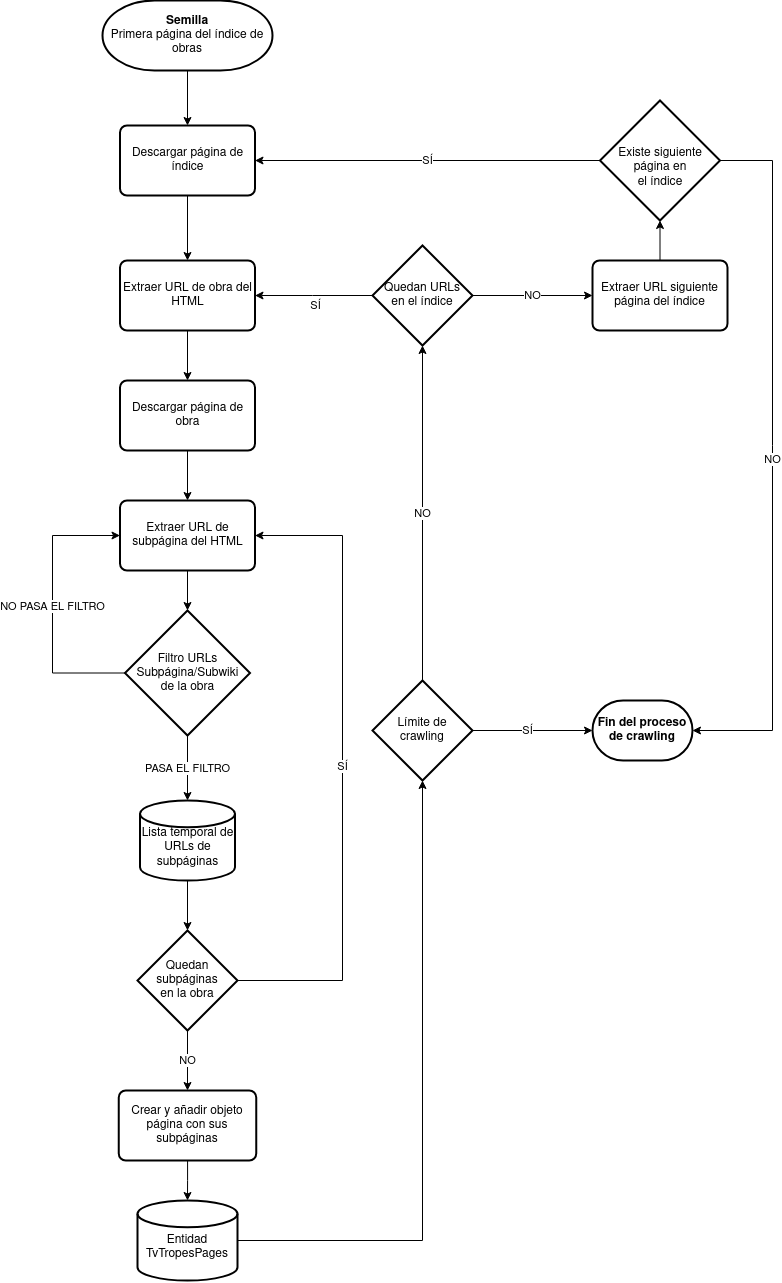
\includegraphics[width=\textwidth]{img/flujo_crawler.png}
    \caption{Diagrama de flujo del funcionamiento del \textit{crawler}.}
    \label{fig:crawling}
\end{figure}

Esto mejora la estrategia de Tropescraper, que encontraba las páginas de
películas a través de referencias en las de \textit{tropos}. En TvTropes no se
puede confiar que una página, de cualquier tipo, liste todos los ejemplos
relacionados. Existen numerosos casos de películas que tienen un \textit{tropo}
concreto, pero que luego no aparecen referenciadas al entrar en la página de ese
\textit{tropo}. Esta relación bidireccional a la cual se ha hecho alusión
en ocasiones anteriores no siempre es cierta, porque aunque técnicamente estén
relacionados, no se puede esperar que los redactores humanos de TvTropes hayan
tenido en cuenta todas las relaciones y referencias en ambas direcciones y las
hayan escrito. Con este índice no solo se mejora por completo el
\textit{crawling} de TvTropes, asegurando que se obtienen todas las obras
registradas sin lugar a duda, sino que simplifica enormemente el proceso al
estar todo organizado en un índice. Además, el \textit{scraping} de Tropescraper
solamente extraía los que están en la sección principal, ignorando los subwikis.

\subsection{Limitación de la carga al servidor de TvTropes}
Como se ha introducido al inicio de este hito, llegados a este punto del
desarrollo es imprescindible tener en cuenta ciertas cuestiones relativas a la
relación entre el bot y la página web y empezar a seguir varias políticas de
cortesía en la implementación. El objetivo es tener una ejecución más eficiente
y que suponga una carga mínima sobre TvTropes, realizando solamente las
operaciones necesarias y sin repetir nada ya extraído, lo cual es imprescindible
al estar ya trabajando con grandes volúmenes de datos. Esto además limitará el
riesgo de que TvTropes ejerza mecanismos anti-\textit{scraping}, como pueden ser
el retraso de peticiones, la denegación de acceso temporal o, lo que sería aún
peor, bloquear el acceso por completo. Se necesitan de mecanismos que permitan
que el programa funcione como un usuario más sin llamar la atención.

Todo este proceso de mejora del \textit{crawler} se basa en las
\href{https://github.com/jlgallego99/TropesToGo/issues/7}{[HU02]} y
\href{https://github.com/jlgallego99/TropesToGo/issues/45}{[HU06]}, que nos
indican que el usuario quiere poder obtener los datos de la forma más rápida
posible y pudiendo elegir no tener la totalidad de los datos existentes. Como
paso previo, se permite elegir limitar el proceso de \textit{crawling} a un
número de obras limitado en lugar de encontrarlas todas. Esto facilitará la
creación de demos y satisfará a aquellos usuarios que necesiten solo de un
subconjunto reducido de los datos, que además reducirá enormemente el tiempo que
el bot tenga que estar trabajando.

\subsubsection{Reutilización de páginas extraídas}
Con la primera versión del \textit{crawler} construida, se realizó una pequeña
demo real sobre TvTropes para comprobar su efectividad. Se consiguieron extraer
más de 500 películas, sin embargo, pasado ese umbral el programa paró de dar
resultados. Al entrar a TvTropes desde un navegador se pudo ver la razón: la web
mostraba una única página con un mensaje indicando que TvTropes detectó un
número alto de peticiones y que esperase unos pocos minutos antes de volver a
intentarlo de nuevo, lo cual puso de manifiesto la necesidad de controlar mucho
mejor las peticiones HTTP enviadas.

Una de las principales razones por las que se llegó a este caso se debía a que
el \textit{crawler} necesita extraer el HTML, teniendo que llevar a cabo, por
tanto, una petición HTTP a la página para ello. Y luego el \textit{scraper}, que
solo tenía los URL de las páginas encontradas por el \textit{crawler}, volvía a
repetir peticiones a esas páginas para volver a obtener sus contenidos, por lo
que cada página de obra se llamaba dos veces, sobrecargando la red más de lo
necesario.

Existen varias soluciones para esto, que pasan por la idea de tener una caché
(temporal o persistida) de los contenidos de las páginas extraídas. Esto se
puede hacer de múltiples maneras: mediante variables en el código,
descargándolas y guardándolas en disco (con la consiguiente pérdida en
eficiencia que supondría escribir y leer tantos ficheros constantemente) o, la
más sofisticada, mediante un servidor \textit{proxy} que redirija las
peticiones, permitiendo a la vez ocultar la fuente de las peticiones y utilizar
la caché de páginas del servidor para no repetir llamadas a TvTropes
\cite{apress2018scraping}.

Como opción mínima viable se decide tener una caché temporal como un campo
adicional en la entidad \texttt{TvTropesPages} la cual es el principal punto de
unión entre \textit{crawler} y \textit{scraper}. Tal y como funciona el
\textit{crawler}, necesita descargar las páginas de cada obra para encontrar las
subpáginas que tengan. En este proceso entra primero una petición HTTP a la
página y luego una transformación a documento Goquery, que es la biblioteca
encargada de poder iterar sobre el árbol de elementos para encontrar lo que se
necesita. Este objeto Goquery es el recurso con el que ambos servicios
encuentran lo que necesitan, ya sea enlaces o metadatos, y es siempre un objeto
referenciado. Por tanto, la solución a este problema se basa en que toda la
carga de realizar las peticiones al servidor recaiga sobre el \textit{crawler},
que al crear cada uno de los objetos \texttt{Page} y añadirlos a la entidad \texttt{TvTropesPages} realizan 
directamente la petición HTTP y transforman el
contenido al documento Goquery, liberando al \textit{scraper} de cualquier tarea
de red. Esto supone una gran mejora en eficiencia del código, escalabilidad y
simplicidad, puesto que basta con reutilizar el documento. El
\textit{scraper} se ahorra dos operaciones bastante costosas y que hasta ahora
se estaban haciendo de forma duplicada: la descarga del HTML y su transformación
a un documento Goquery, con el consiguiente duplicado de variables y desperdicio
de espacio en memoria que suponía. Ahora, una vez que se ha visitado una página,
no se volverá a visitar durante la misma ejecución, ya que ya está descargada.

\subsubsection{Limitación de la tasa de crawling}
La solución anterior ya supone una gran mejora en eficiencia y en controlar
mejor las peticiones, sin embargo, aún quedan consideraciones a tener en cuenta
en el ámbito del \textit{scraping} para poder limitar y esconder mejor el bot.
Se deben tener en cuenta políticas de cortesía con respecto a las peticiones que
se hace a la web, y la más común y efectiva de ellas es limitar la tasa de
\textit{crawling} aleatoriamente \cite{apress2018scraping}. Esto consiste
simplemente en dejar el programa en esperas aleatorias entre petición y
petición, pero no demasiado largas como para que sean negativas para el
desempeño del bot. Se implementa una espera aleatoria de máximo 1 segundo entre
cada petición, lo suficiente para que el bucle de peticiones no sobrecargue de
peticiones al servidor en un corto periodo de tiempo, y también para que no sean
predecibles y sufrir el riesgo de ser bloqueados. También se estudian
los códigos de error que devuelve TvTropes, y si son códigos como 403, que
indican que se ha denegado el acceso como en la demo que se hizo, se realiza una
espera mayor hasta que se levante la restricción y poder continuar.

Con estos cambios, ambos servicios son ya capaces de ejecutar un gran número de
peticiones y extracciones de datos más eficientemente y respetando al
servidor de TvTropes. Sin embargo, en el ámbito del \textit{scraping} es
necesario tener siempre una capa extra de seguridad, por lo que es muy
recomendable hacer más robusto al bot para que pase desapercibido. Uno de
los aspectos que más debe tener en cuenta cualquier \textit{scraper}, como se
dijo en el \autoref{chapter:3}, es modificar las cabeceras de las peticiones
HTTP con información típica que contienen los navegadores para evitar ser
rechazados al instante por no ser un usuario humano \cite{apress2018scraping}.
Las más importantes son la cabecera \texttt{User-Agent} con la información de un
navegador o la cabecera \texttt{Referer} con la URL de donde se supone que
procede la petición. Se opta por poner que las peticiones proceden de un
navegador Firefox, que es bastante común, y referidas desde Google, ya que es
bastante común e improbable que se bloquee una petición que provenga desde ahí
\cite{bettenbuk_10_2019}.

También es recomendable añadir otras cabeceras adicionales que suelen añadir los
navegadores, las cuales son de muchos tipos. Se utilizan las proporcionadas por
la web \texttt{HTTPBin} en uno de sus
ejemplos\footnote{\url{https://httpbin.org/anything}}, una web recomendable para
hacer pruebas HTTP de cualquier tipo \cite{bettenbuk_10_2019}.

TvTropes no es una página que tenga demasiados mecanismos en contra de los
\textit{scrapers} por completo, más allá de poner limitaciones cuando les
llueven muchas peticiones desde una misma IP, sin embargo, nunca sobra tener un
poco más de precaución.

Estas mejoras para intentar limitar la carga de TvTropes constituyen un parche
que mejora la eficiencia y protege al \textit{scraper} contra posibles
denegaciones por parte de TvTropes, por lo que siguiendo el versionado semántico
se aumenta la última versión, teniendo al final de este PMV una versión 0.5.1 de
TropesToGo.

\section{Extracción de otros medios audiovisuales}
\section{Resultado final}